%%%%%%%%%%%%%%%%%%%%%%%%%%%%%%%%%%%%%%%%%
% Programming/Coding Assignment
% LaTeX Template
%
% This template has been downloaded from:
% http://www.latextemplates.com
%
% Original author:
% Ted Pavlic (http://www.tedpavlic.com)
%
% Note:
% The \lipsum[#] commands throughout this template generate dummy text
% to fill the template out. These commands should all be removed when 
% writing assignment content.
%
% This template uses a Perl script as an example snippet of code, most other
% languages are also usable. Configure them in the "CODE INCLUSION 
% CONFIGURATION" section.
%
%%%%%%%%%%%%%%%%%%%%%%%%%%%%%%%%%%%%%%%%%

%----------------------------------------------------------------------------------------
%	PACKAGES AND OTHER DOCUMENT CONFIGURATIONS
%----------------------------------------------------------------------------------------

\documentclass{article}

\usepackage{fancyhdr} % Required for custom headers
\usepackage{lastpage} % Required to determine the last page for the footer
\usepackage{extramarks} % Required for headers and footers
\usepackage[usenames,dvipsnames]{color} % Required for custom colors
\usepackage{graphicx} % Required to insert images
\usepackage{listings} % Required for insertion of code
\usepackage{courier} % Required for the courier font
\usepackage{lipsum} % Used for inserting dummy 'Lorem ipsum' text into the template

\usepackage{float}
\usepackage{amsfonts}
\usepackage{amsmath}
\usepackage{bm}

% Margins
\topmargin=-0.45in
\evensidemargin=0in
\oddsidemargin=0in
\textwidth=6.5in
\textheight=9.0in
\headsep=0.25in

\linespread{1.1} % Line spacing

% Set up the header and footer
\pagestyle{fancy}
\lhead{K. Holmbeck and D. Tonne} % Top left header
\chead{\hmwkClass\ : \hmwkTitle} % Top center head
\rhead{\firstxmark} % Top right header
\lfoot{\lastxmark} % Bottom left footer
\cfoot{} % Bottom center footer
\rfoot{Page\ \thepage\ of\ \pageref{LastPage}} % Bottom right footer
\renewcommand\headrulewidth{0.4pt} % Size of the header rule
\renewcommand\footrulewidth{0.4pt} % Size of the footer rule

\setlength\parindent{0pt} % Removes all indentation from paragraphs

%----------------------------------------------------------------------------------------
%	CODE INCLUSION CONFIGURATION
%----------------------------------------------------------------------------------------

\usepackage{color} %red, green, blue, yellow, cyan, magenta, black, white
\definecolor{mygreen}{RGB}{28,172,0} % color values Red, Green, Blue
\definecolor{mylilas}{RGB}{170,55,241}

\lstset{language=Matlab,%
    basicstyle=\ttfamily\footnotesize,breaklines=true
    %basicstyle=\footnotesize\color{red},
    breaklines=true,%
    xleftmargin=0.5in,
    %xrightmargin=0.25in,
    morekeywords={matlab2tikz},
    keywordstyle=\color{blue},%
    morekeywords=[2]{1}, keywordstyle=[2]{\color{black}},
    identifierstyle=\color{black},%
    stringstyle=\color{mylilas},
    commentstyle=\color{mygreen},%
    showstringspaces=false,%without this there will be a symbol in the places where there is a space
    numbers=left,%
    numberstyle={\tiny \color{black}},% size of the numbers
    numbersep=9pt, % this defines how far the numbers are from the text
    emph=[1]{for,end,break},emphstyle=[1]\color{blue}, %some words to emphasise
    %emph=[2]{word1,word2}, emphstyle=[2]{style},    
}


%----------------------------------------------------------------------------------------
%	DOCUMENT STRUCTURE COMMANDS
%	Skip this unless you know what you're doing
%----------------------------------------------------------------------------------------

% Header and footer for when a page split occurs within a problem environment
\newcommand{\enterProblemHeader}[1]{
%\nobreak\extramarks{#1}{#1 continued on next page\ldots}\nobreak
%\nobreak\extramarks{#1 (continued)}{#1 continued on next page\ldots}\nobreak
}

% Header and footer for when a page split occurs between problem environments
\newcommand{\exitProblemHeader}[1]{
\nobreak\extramarks{#1 (continued)}{#1 continued on next page\ldots}\nobreak
\nobreak\extramarks{#1}{}\nobreak
}

\setcounter{secnumdepth}{0} % Removes default section numbers
\newcounter{homeworkProblemCounter} % Creates a counter to keep track of the number of problems

\newcommand{\homeworkProblemName}{}
\newenvironment{homeworkProblem}[1][Problem \arabic{homeworkProblemCounter}]{ % Makes a new environment called homeworkProblem which takes 1 argument (custom name) but the default is "Problem #"
\stepcounter{homeworkProblemCounter} % Increase counter for number of problems
\renewcommand{\homeworkProblemName}{#1} % Assign \homeworkProblemName the name of the problem
\subsection{\homeworkProblemName} % Make a section in the document with the custom problem count
\enterProblemHeader{\homeworkProblemName} % Header and footer within the environment
}{
\exitProblemHeader{\homeworkProblemName} % Header and footer after the environment
}

\newcommand{\problemAnswer}[1]{ % Defines the problem answer command with the content as the only argument
\noindent\framebox[\columnwidth][c]{\begin{minipage}{0.98\columnwidth}#1\end{minipage}} % Makes the box around the problem answer and puts the content inside
}

\newcommand{\homeworkSectionName}{}
\newenvironment{homeworkSection}[1]{ % New environment for sections within homework problems, takes 1 argument - the name of the section
\renewcommand{\homeworkSectionName}{#1} % Assign \homeworkSectionName to the name of the section from the environment argument
\subsection{\homeworkSectionName} % Make a subsection with the custom name of the subsection
\enterProblemHeader{\homeworkProblemName\ [\homeworkSectionName]} % Header and footer within the environment
}{
\enterProblemHeader{\homeworkProblemName} % Header and footer after the environment
}


%----------------------------------------------------------------------------------------
%	NAME AND CLASS SECTION
%----------------------------------------------------------------------------------------

\newcommand{\hmwkTitle}{Homework\ 1} % Assignment title
\newcommand{\hmwkDueDate}{Thursday,\ February\ 15,\ 2018} % Due date
\newcommand{\hmwkClass}{Math\ 521} % Course/clas
\newcommand{\hmwkAuthorName}{Kristin Holmbeck} % Your name

%----------------------------------------------------------------------------------------
%	TITLE PAGE
%----------------------------------------------------------------------------------------

\title{
\vspace{2in}
\textmd{\textbf{\hmwkClass:\ \hmwkTitle}}\\
\normalsize\vspace{0.1in}\small{Due\ on\ \hmwkDueDate}\\
\vspace{0.1in}
\vspace{3in}
}

\author{\textbf{\hmwkAuthorName}}
\date{} % Insert date here if you want it to appear below your name

%----------------------------------------------------------------------------------------

\begin{document}

\maketitle

%----------------------------------------------------------------------------------------
%	TABLE OF CONTENTS
%----------------------------------------------------------------------------------------

%\setcounter{tocdepth}{1} % Uncomment this line if you don't want subsections listed in the ToC

\newpage
\tableofcontents
\listoffigures
\newpage

%----------------------------------------------------------------------------------------
%	PROBLEM 1
%----------------------------------------------------------------------------------------

% To have just one problem per page, simply put a \clearpage after each problem

\begin{section}{Theory}

\begin{homeworkSection}{Change of Basis}

Let the basis $\mathcal{B}_1$ be the standard basis in $\mathbb{R}^2$, i.e., $\mathcal{B}_1 = span \left \{ \Vec{e_1}, \Vec{e_2} \right \}$, 
and the basis $\mathcal{B}_2$ be given by 
 $\mathcal{B}_2 = span \left \{\begin{bmatrix}1 \\ 1\end{bmatrix} , \begin{bmatrix} -1 \\ 1\end{bmatrix} \right \}$. Given $u_{\mathcal{B}_1} = (1, 1)^T$, find $u_{\mathcal{B}_2}$.

\problemAnswer{
\begin{align*}
    V = \begin{bmatrix} 1 & 0 \\ 0 & 1 \end{bmatrix} &,
    W = \begin{bmatrix} 1 & -1 \\ 1 & 1 \end{bmatrix} 
    \implies  W^{-1} = \frac{1}{2} \begin{bmatrix} 1 & 1 \\ -1 & 1 \end{bmatrix} \\
    u_{\mathcal{B}_2} &= W^{-1}V u_{\mathcal{B}_1} 
        = \begin{bmatrix} 1 \\ 0 \end{bmatrix}
\end{align*}
}
\end{homeworkSection}

\end{section}

%----------------------------------------------------------------------------------------
%	PROBLEM 2
%----------------------------------------------------------------------------------------
\begin{section}{Computing}

\begin{homeworkSection}{Unit Circle Transformations}
Write a code to generate 1000 random numbers contained on the unit circle. Apply several random matrices to this data and describe your results in the terminology of bases and change of bases. How do your results differ if the multiplying matrix is constrained to be orthogonal?
 \\
 
The following matrices are the transformations used in Figure \ref{fig:unitCirc}, and note that $A_3$ is the $Q$ matrix for the QR decomposition of $A_1$.

\begin{align*}
    A_1 = \begin{bmatrix} 0.524 && -0.038 \\ -0.401 && -0.210 \end{bmatrix}, \quad
    A_2 = \begin{bmatrix} 2 && 0 \\ 0 && 2 \end{bmatrix}, \quad
    A_3 = \begin{bmatrix} -0.794 && 0.608 \\ 0.608 && 0.794\end{bmatrix}
\end{align*}
 
\begin{figure}[H]
\centering
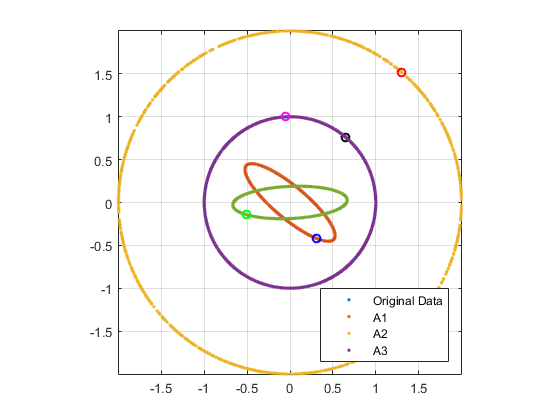
\includegraphics[width=0.75\columnwidth]{../data/rand_unit_circ_pts} % Example image
\caption{Transformation of Points on the Unit Circle}
\label{fig:unitCirc}
\end{figure}

The actual data lies underneath the orthogonal, or $A_3$-transformed data on the graph. That is, the orthogonal transformation rotated the unit circle counter-clockwise. As expected, the scaling matrix $A_2$ uniformly scaled the points outwards (since the scaling factor was greater than 1). 
\\

The random matrix, $A_1$, scaled the unit circle non-uniformly into an ellipse. For extra fun, applying the orthogonal transformation to these elliptically-scaled points simply rotated the matrix. 

\problemAnswer{

}
\end{homeworkSection}


\begin{homeworkSection}{Principal Angles}
\end{homeworkSection}


\begin{homeworkSection}{Image Transformations}

Any linear transformation i $\mathbb{R}^2$ is represented with respect to homogeneous coordinates by a matrix of the form:

$$
    \begin{bmatrix}
        A_{2 x 2} && \mathbf{0} \\ \mathbf{0}  && \mathbf{1}
    \end{bmatrix}
$$

Image translation is simple, as every point is uniformly translated in either direction. For scaling and rotation, however, using a matrix of the form above is necessary. \\

For the following images, we used \textsc{Matlab}'s built-in image demo, coins.png (Figure \ref{fig:orig}).

\begin{figure}[!h]
\centering
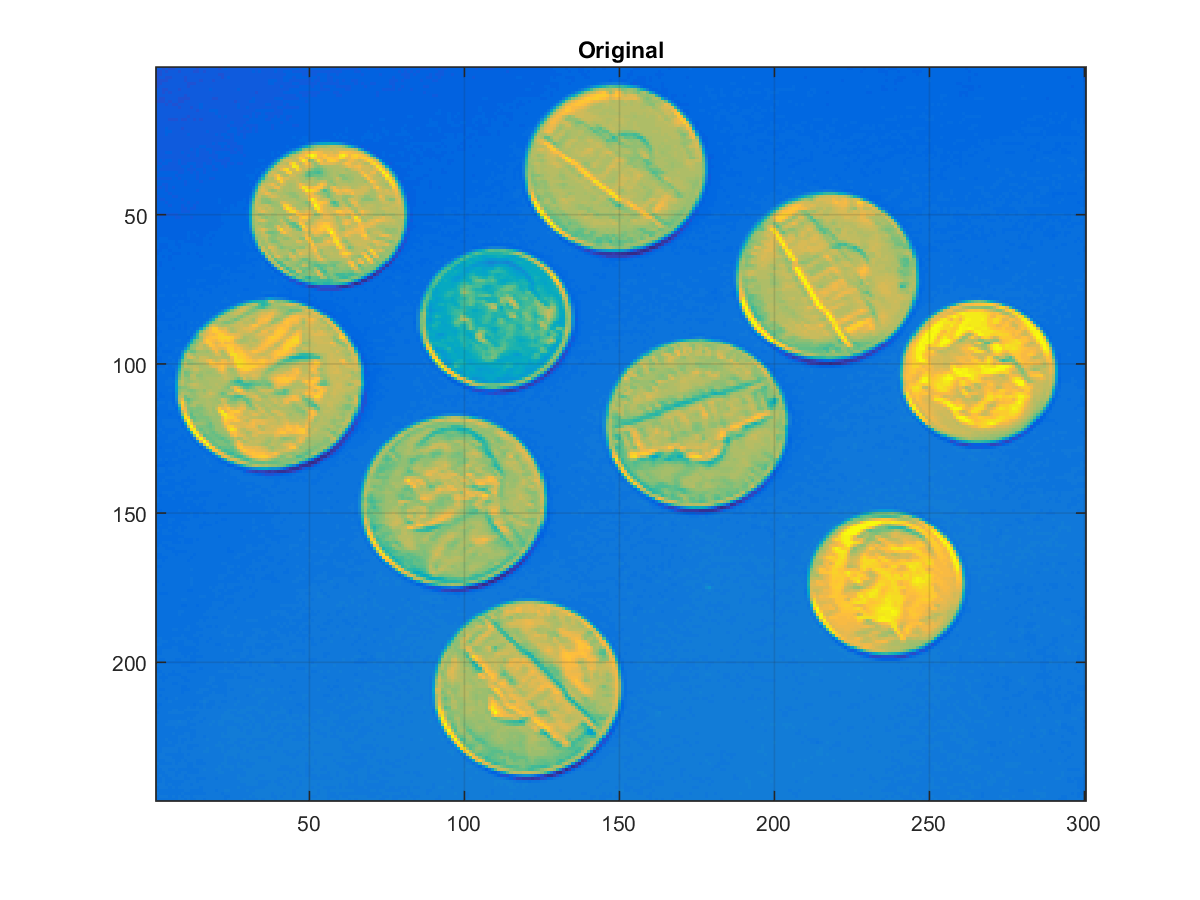
\includegraphics[width=0.75\columnwidth]{../data/orig} % Example image
\caption{\textsc{Matlab}'s coins.png}
\label{fig:orig}
\end{figure}


\begin{subsubsection}{Scaling}

As shown in class, for scaling by $s_x$ and $s_y$ in the $x-$ and $y-$directions respectively, the corresponding scaling transformation matrix is given by

\begin{align*}
    M_{scale}(p) = \begin{bmatrix} s_x && 0 && (1-s_x)t_x \\
        0 && s_y && (1-s_y)t_y \\
        0 && 0 && 1 \end{bmatrix}
\end{align*}

where $p = \begin{bmatrix} t_x && t_y && 1 \end{bmatrix}^T$. 
The data in Figure \ref{fig:scaled} was scaled by 2 in both $x$ and $y$, about the point $(t_x, t_y) = (150, 50)$. 

\begin{figure}[!h]
\centering
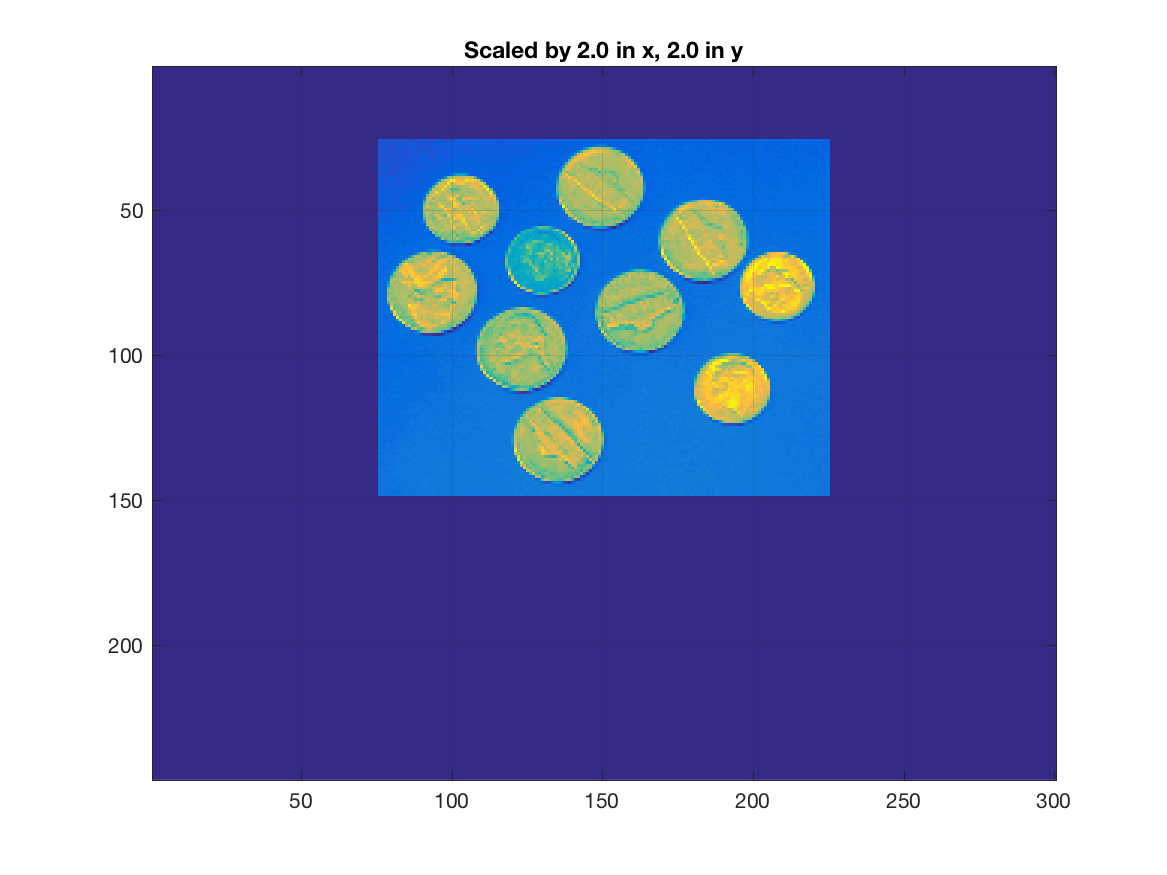
\includegraphics[width=0.75\columnwidth]{../data/scaled} % Example image
\caption{Image scaling about a point}
\label{fig:scaled}
\end{figure}
\end{subsubsection}


\begin{subsubsection}{Translation}
\end{subsubsection}


\begin{subsubsection}{Rotation}

As shown in class, for rotating by $\theta$ about a point $p = \begin{bmatrix} t_x && t_y && 1 \end{bmatrix}^T$, the rotation matrix is given by:

\begin{align*}
    M_{rot}(p) = \begin{bmatrix} \cos \theta && -\sin\theta && 0 \\
        \sin\theta && \cos\theta && 0 \\
        0 && 0 && 1 \end{bmatrix}
\end{align*}

So where do we account for $p$? The matrix above rotates points with respect to the origin. In this case, we can translate the image (preserving the entirety of the image, unlike the previous section) by $-p$, which will make the origin $p$. Rotate about the origin, then undo the $-p$ translation by $p$, yielding the desired image.
\\

The data in Figure \ref{fig:scaled} was rotated by $\theta = \pi/2$, about the point $(t_x, t_y) = (150, 50)$. 

\begin{figure}[!h]
\centering
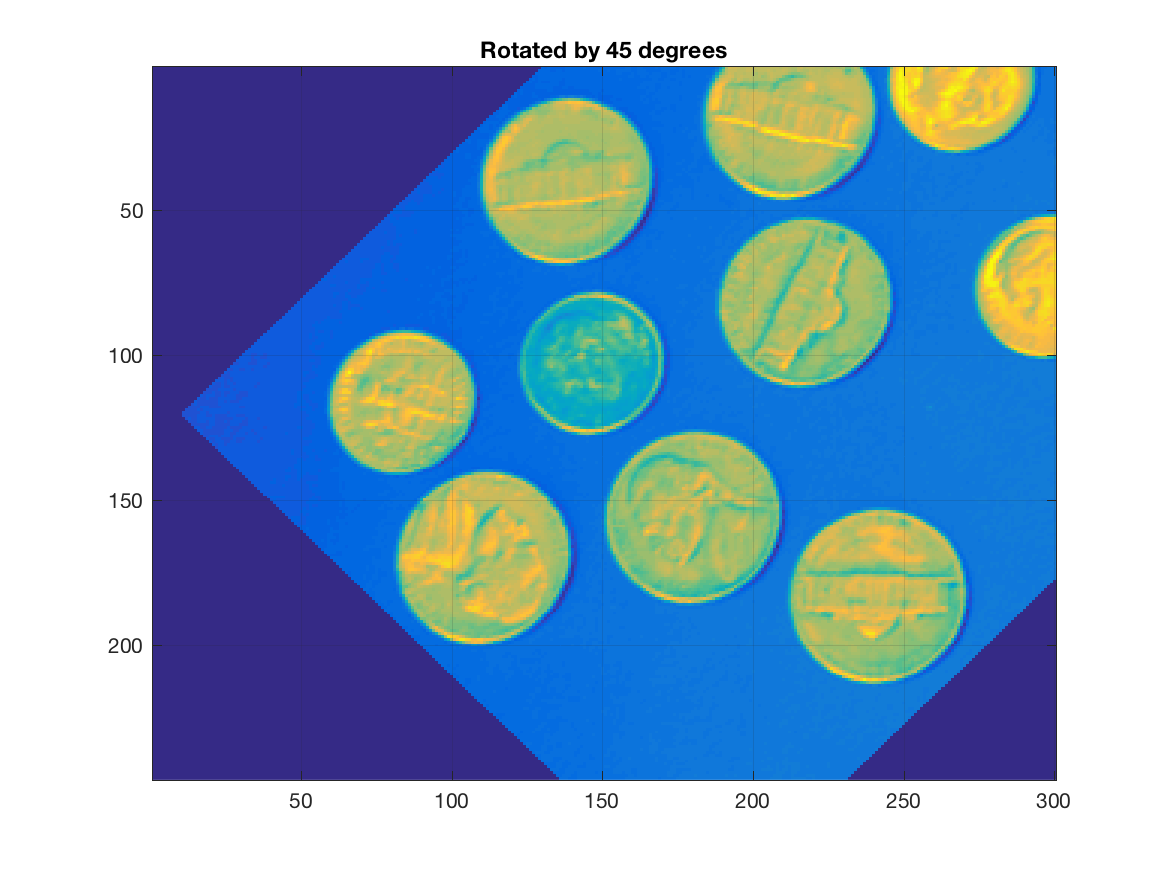
\includegraphics[width=0.75\columnwidth]{../data/rotated} % Example image
\caption{Rotation about a point}
\label{fig:rotated}
\end{figure}
\end{subsubsection}

\end{homeworkSection}



\end{section}



%----------------------------------------------------------------------------------------
\newpage

\appendix

\section{Code}

\subsection{prinAngles.m}

\lstinputlisting{../prinAngles.m}


\subsection{scale.m}
\lstinputlisting{../scale.m}

\subsection{rotate.m}
\lstinputlisting{../rotate.m}

\subsection{translateH.m}
\lstinputlisting{../translateH.m}

\subsection{translateV.m}
\lstinputlisting{../translateV.m}

\end{document}